\documentclass[1p]{elsarticle_modified}
%\bibliographystyle{elsarticle-num}

%\usepackage[colorlinks]{hyperref}
%\usepackage{abbrmath_seonhwa} %\Abb, \Ascr, \Acal ,\Abf, \Afrak
\usepackage{amsfonts}
\usepackage{amssymb}
\usepackage{amsmath}
\usepackage{amsthm}
\usepackage{scalefnt}
\usepackage{amsbsy}
\usepackage{kotex}
\usepackage{caption}
\usepackage{subfig}
\usepackage{color}
\usepackage{graphicx}
\usepackage{xcolor} %% white, black, red, green, blue, cyan, magenta, yellow
\usepackage{float}
\usepackage{setspace}
\usepackage{hyperref}

\usepackage{tikz}
\usetikzlibrary{arrows}

\usepackage{multirow}
\usepackage{array} % fixed length table
\usepackage{hhline}

%%%%%%%%%%%%%%%%%%%%%
\makeatletter
\renewcommand*\env@matrix[1][\arraystretch]{%
	\edef\arraystretch{#1}%
	\hskip -\arraycolsep
	\let\@ifnextchar\new@ifnextchar
	\array{*\c@MaxMatrixCols c}}
\makeatother %https://tex.stackexchange.com/questions/14071/how-can-i-increase-the-line-spacing-in-a-matrix
%%%%%%%%%%%%%%%

\usepackage[normalem]{ulem}

\newcommand{\msout}[1]{\ifmmode\text{\sout{\ensuremath{#1}}}\else\sout{#1}\fi}
%SOURCE: \msout is \stkout macro in https://tex.stackexchange.com/questions/20609/strikeout-in-math-mode

\newcommand{\cancel}[1]{
	\ifmmode
	{\color{red}\msout{#1}}
	\else
	{\color{red}\sout{#1}}
	\fi
}

\newcommand{\add}[1]{
	{\color{blue}\uwave{#1}}
}

\newcommand{\replace}[2]{
	\ifmmode
	{\color{red}\msout{#1}}{\color{blue}\uwave{#2}}
	\else
	{\color{red}\sout{#1}}{\color{blue}\uwave{#2}}
	\fi
}

\newcommand{\Sol}{\mathcal{S}} %segment
\newcommand{\D}{D} %diagram
\newcommand{\A}{\mathcal{A}} %arc


%%%%%%%%%%%%%%%%%%%%%%%%%%%%%5 test

\def\sl{\operatorname{\textup{SL}}(2,\Cbb)}
\def\psl{\operatorname{\textup{PSL}}(2,\Cbb)}
\def\quan{\mkern 1mu \triangleright \mkern 1mu}

\theoremstyle{definition}
\newtheorem{thm}{Theorem}[section]
\newtheorem{prop}[thm]{Proposition}
\newtheorem{lem}[thm]{Lemma}
\newtheorem{ques}[thm]{Question}
\newtheorem{cor}[thm]{Corollary}
\newtheorem{defn}[thm]{Definition}
\newtheorem{exam}[thm]{Example}
\newtheorem{rmk}[thm]{Remark}
\newtheorem{alg}[thm]{Algorithm}

\newcommand{\I}{\sqrt{-1}}
\begin{document}

%\begin{frontmatter}
%
%\title{Boundary parabolic representations of knots up to 8 crossings}
%
%%% Group authors per affiliation:
%\author{Yunhi Cho} 
%\address{Department of Mathematics, University of Seoul, Seoul, Korea}
%\ead{yhcho@uos.ac.kr}
%
%
%\author{Seonhwa Kim} %\fnref{s_kim}}
%\address{Center for Geometry and Physics, Institute for Basic Science, Pohang, 37673, Korea}
%\ead{ryeona17@ibs.re.kr}
%
%\author{Hyuk Kim}
%\address{Department of Mathematical Sciences, Seoul National University, Seoul 08826, Korea}
%\ead{hyukkim@snu.ac.kr}
%
%\author{Seokbeom Yoon}
%\address{Department of Mathematical Sciences, Seoul National University, Seoul, 08826,  Korea}
%\ead{sbyoon15@snu.ac.kr}
%
%\begin{abstract}
%We find all boundary parabolic representation of knots up to 8 crossings.
%
%\end{abstract}
%\begin{keyword}
%    \MSC[2010] 57M25 
%\end{keyword}
%
%\end{frontmatter}

%\linenumbers
%\tableofcontents
%
\newcommand\colored[1]{\textcolor{white}{\rule[-0.35ex]{0.8em}{1.4ex}}\kern-0.8em\color{red} #1}%
%\newcommand\colored[1]{\textcolor{white}{ #1}\kern-2.17ex	\textcolor{white}{ #1}\kern-1.81ex	\textcolor{white}{ #1}\kern-2.15ex\color{red}#1	}

{\Large $\underline{11n_{2}~(K11n_{2})}$}

\setlength{\tabcolsep}{10pt}
\renewcommand{\arraystretch}{1.6}
\vspace{1cm}\begin{tabular}{m{100pt}>{\centering\arraybackslash}m{274pt}}
\multirow{5}{120pt}{
	\centering
	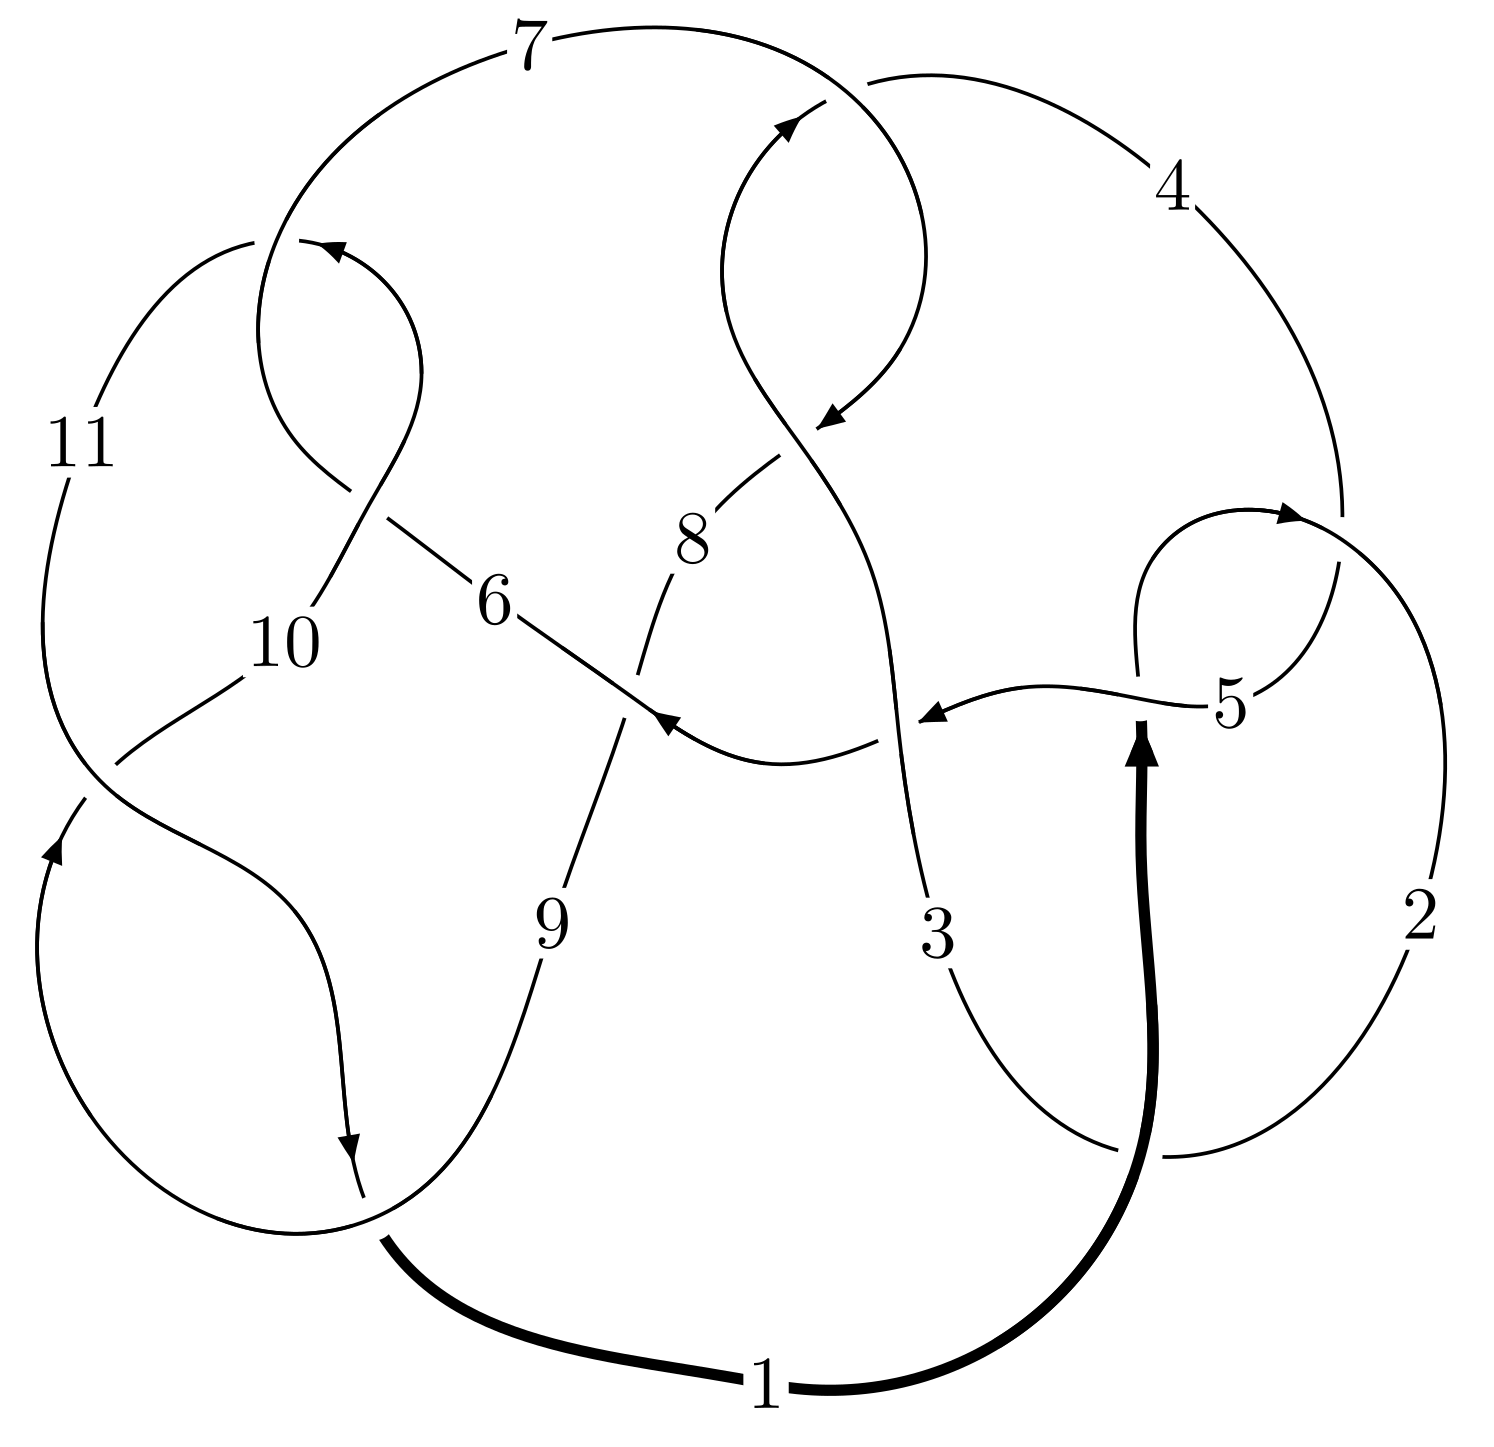
\includegraphics[width=112pt]{../../../GIT/diagram.site/Diagrams/png/618_11n_2.png}\\
\ \ \ A knot diagram\footnotemark}&
\allowdisplaybreaks
\textbf{Linearized knot diagam} \\
\cline{2-2}
 &
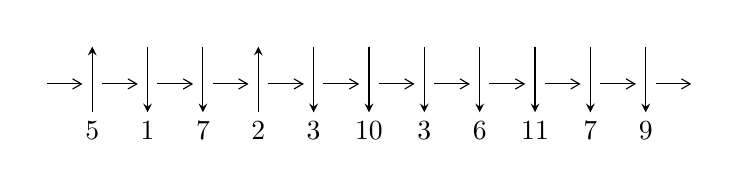
\begin{tikzpicture}[x=20pt, y=17pt]
	% nodes
	\node (C0) at (0, 0) {};
	\node (C1) at (1, 0) {};
	\node (C1U) at (1, +1) {};
	\node (C1D) at (1, -1) {5};

	\node (C2) at (2, 0) {};
	\node (C2U) at (2, +1) {};
	\node (C2D) at (2, -1) {1};

	\node (C3) at (3, 0) {};
	\node (C3U) at (3, +1) {};
	\node (C3D) at (3, -1) {7};

	\node (C4) at (4, 0) {};
	\node (C4U) at (4, +1) {};
	\node (C4D) at (4, -1) {2};

	\node (C5) at (5, 0) {};
	\node (C5U) at (5, +1) {};
	\node (C5D) at (5, -1) {3};

	\node (C6) at (6, 0) {};
	\node (C6U) at (6, +1) {};
	\node (C6D) at (6, -1) {10};

	\node (C7) at (7, 0) {};
	\node (C7U) at (7, +1) {};
	\node (C7D) at (7, -1) {3};

	\node (C8) at (8, 0) {};
	\node (C8U) at (8, +1) {};
	\node (C8D) at (8, -1) {6};

	\node (C9) at (9, 0) {};
	\node (C9U) at (9, +1) {};
	\node (C9D) at (9, -1) {11};

	\node (C10) at (10, 0) {};
	\node (C10U) at (10, +1) {};
	\node (C10D) at (10, -1) {7};

	\node (C11) at (11, 0) {};
	\node (C11U) at (11, +1) {};
	\node (C11D) at (11, -1) {9};
	\node (C12) at (12, 0) {};

	% arrows
	\draw[->,>={angle 60}]
	(C0) edge (C1) (C1) edge (C2) (C2) edge (C3) (C3) edge (C4) (C4) edge (C5) (C5) edge (C6) (C6) edge (C7) (C7) edge (C8) (C8) edge (C9) (C9) edge (C10) (C10) edge (C11) (C11) edge (C12) ;	\draw[->,>=stealth]
	(C1D) edge (C1U) (C2U) edge (C2D) (C3U) edge (C3D) (C4D) edge (C4U) (C5U) edge (C5D) (C6U) edge (C6D) (C7U) edge (C7D) (C8U) edge (C8D) (C9U) edge (C9D) (C10U) edge (C10D) (C11U) edge (C11D) ;
	\end{tikzpicture} \\
\hhline{~~} \\& 
\textbf{Solving Sequence} \\ \cline{2-2} 
 &
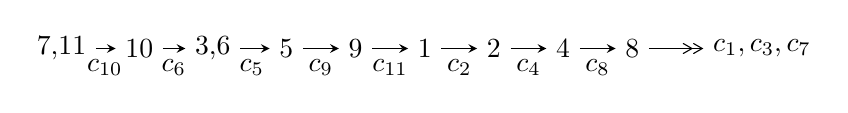
\begin{tikzpicture}[x=25pt, y=7pt]
	% node
	\node (A0) at (-1/8, 0) {7,11};
	\node (A1) at (1, 0) {10};
	\node (A2) at (33/16, 0) {3,6};
	\node (A3) at (25/8, 0) {5};
	\node (A4) at (33/8, 0) {9};
	\node (A5) at (41/8, 0) {1};
	\node (A6) at (49/8, 0) {2};
	\node (A7) at (57/8, 0) {4};
	\node (A8) at (65/8, 0) {8};
	\node (C1) at (1/2, -1) {$c_{10}$};
	\node (C2) at (3/2, -1) {$c_{6}$};
	\node (C3) at (21/8, -1) {$c_{5}$};
	\node (C4) at (29/8, -1) {$c_{9}$};
	\node (C5) at (37/8, -1) {$c_{11}$};
	\node (C6) at (45/8, -1) {$c_{2}$};
	\node (C7) at (53/8, -1) {$c_{4}$};
	\node (C8) at (61/8, -1) {$c_{8}$};
	\node (A9) at (10, 0) {$c_{1},c_{3},c_{7}$};

	% edge
	\draw[->,>=stealth]	
	(A0) edge (A1) (A1) edge (A2) (A2) edge (A3) (A3) edge (A4) (A4) edge (A5) (A5) edge (A6) (A6) edge (A7) (A7) edge (A8) ;
	\draw[->>,>={angle 60}]	
	(A8) edge (A9);
\end{tikzpicture} \\ 

\end{tabular} \\

\footnotetext{
The image of knot diagram is generated by the software ``\textbf{Draw programme}" developed by Andrew Bartholomew(\url{http://www.layer8.co.uk/maths/draw/index.htm\#Running-draw}), where we modified some parts for our purpose(\url{https://github.com/CATsTAILs/LinksPainter}).
}\phantom \\ \newline 
\centering \textbf{Ideals for irreducible components\footnotemark of $X_{\text{par}}$} 
 
\begin{align*}
I^u_{1}&=\langle 
-2 u^{33}-5 u^{32}+\cdots+2 b- u,\;-2 u^{33}-4 u^{32}+\cdots+a+1,\;u^{34}+3 u^{33}+\cdots+3 u^2-1\rangle \\
I^u_{2}&=\langle 
- u^2 b+b^2+b u- u+1,\;a,\;u^3- u^2+1\rangle \\
\\
\end{align*}
\raggedright * 2 irreducible components of $\dim_{\mathbb{C}}=0$, with total 40 representations.\\
\footnotetext{All coefficients of polynomials are rational numbers. But the coefficients are sometimes approximated in decimal forms when there is not enough margin.}
\newpage
\renewcommand{\arraystretch}{1}
\centering \section*{I. $I^u_{1}= \langle -2 u^{33}-5 u^{32}+\cdots+2 b- u,\;-2 u^{33}-4 u^{32}+\cdots+a+1,\;u^{34}+3 u^{33}+\cdots+3 u^2-1 \rangle$}
\flushleft \textbf{(i) Arc colorings}\\
\begin{tabular}{m{7pt} m{180pt} m{7pt} m{180pt} }
\flushright $a_{7}=$&$\begin{pmatrix}0\\u\end{pmatrix}$ \\
\flushright $a_{11}=$&$\begin{pmatrix}1\\0\end{pmatrix}$ \\
\flushright $a_{10}=$&$\begin{pmatrix}1\\- u^2\end{pmatrix}$ \\
\flushright $a_{3}=$&$\begin{pmatrix}2 u^{33}+4 u^{32}+\cdots+2 u-1\\u^{33}+\frac{5}{2} u^{32}+\cdots-2 u^2+\frac{1}{2} u\end{pmatrix}$ \\
\flushright $a_{6}=$&$\begin{pmatrix}u\\- u^3+u\end{pmatrix}$ \\
\flushright $a_{5}=$&$\begin{pmatrix}- u^4+u^2-1\\-\frac{1}{2} u^{32}- u^{31}+\cdots+3 u^2+\frac{3}{2} u\end{pmatrix}$ \\
\flushright $a_{9}=$&$\begin{pmatrix}- u^2+1\\- u^2\end{pmatrix}$ \\
\flushright $a_{1}=$&$\begin{pmatrix}u^4- u^2+1\\u^4\end{pmatrix}$ \\
\flushright $a_{2}=$&$\begin{pmatrix}\frac{1}{2} u^{33}+u^{32}+\cdots+2 u+\frac{1}{2}\\\frac{1}{2} u^{33}+4 u^{32}+\cdots+4 u-2\end{pmatrix}$ \\
\flushright $a_{4}=$&$\begin{pmatrix}-2 u^{33}-4 u^{32}+\cdots-2 u+1\\-2 u^{33}-\frac{11}{2} u^{32}+\cdots-\frac{5}{2} u+2\end{pmatrix}$ \\
\flushright $a_{8}=$&$\begin{pmatrix}- u^6+u^4-2 u^2+1\\u^8-2 u^6+2 u^4-2 u^2\end{pmatrix}$\\ \flushright $a_{8}=$&$\begin{pmatrix}- u^6+u^4-2 u^2+1\\u^8-2 u^6+2 u^4-2 u^2\end{pmatrix}$\\&\end{tabular}
\flushleft \textbf{(ii) Obstruction class $= -1$}\\~\\
\flushleft \textbf{(iii) Cusp Shapes $= \frac{17}{2} u^{33}+19 u^{32}+\cdots+10 u-\frac{25}{2}$}\\~\\
\newpage\renewcommand{\arraystretch}{1}
\flushleft \textbf{(iv) u-Polynomials at the component}\newline \\
\begin{tabular}{m{50pt}|m{274pt}}
Crossings & \hspace{64pt}u-Polynomials at each crossing \\
\hline $$\begin{aligned}c_{1},c_{4}\end{aligned}$$&$\begin{aligned}
&u^{34}+4 u^{33}+\cdots+7 u+1
\end{aligned}$\\
\hline $$\begin{aligned}c_{2}\end{aligned}$$&$\begin{aligned}
&u^{34}+20 u^{33}+\cdots-31 u+1
\end{aligned}$\\
\hline $$\begin{aligned}c_{3},c_{7}\end{aligned}$$&$\begin{aligned}
&u^{34}+u^{33}+\cdots-160 u-64
\end{aligned}$\\
\hline $$\begin{aligned}c_{5}\end{aligned}$$&$\begin{aligned}
&u^{34}-4 u^{33}+\cdots+19 u+2
\end{aligned}$\\
\hline $$\begin{aligned}c_{6},c_{10}\end{aligned}$$&$\begin{aligned}
&u^{34}+3 u^{33}+\cdots+3 u^2-1
\end{aligned}$\\
\hline $$\begin{aligned}c_{8}\end{aligned}$$&$\begin{aligned}
&u^{34}-3 u^{33}+\cdots+4 u-1
\end{aligned}$\\
\hline $$\begin{aligned}c_{9},c_{11}\end{aligned}$$&$\begin{aligned}
&u^{34}+13 u^{33}+\cdots+6 u+1
\end{aligned}$\\
\hline
\end{tabular}\\~\\
\newpage\renewcommand{\arraystretch}{1}
\flushleft \textbf{(v) Riley Polynomials at the component}\newline \\
\begin{tabular}{m{50pt}|m{274pt}}
Crossings & \hspace{64pt}Riley Polynomials at each crossing \\
\hline $$\begin{aligned}c_{1},c_{4}\end{aligned}$$&$\begin{aligned}
&y^{34}+20 y^{33}+\cdots-31 y+1
\end{aligned}$\\
\hline $$\begin{aligned}c_{2}\end{aligned}$$&$\begin{aligned}
&y^{34}-8 y^{33}+\cdots-1215 y+1
\end{aligned}$\\
\hline $$\begin{aligned}c_{3},c_{7}\end{aligned}$$&$\begin{aligned}
&y^{34}-35 y^{33}+\cdots-29696 y+4096
\end{aligned}$\\
\hline $$\begin{aligned}c_{5}\end{aligned}$$&$\begin{aligned}
&y^{34}-36 y^{33}+\cdots-209 y+4
\end{aligned}$\\
\hline $$\begin{aligned}c_{6},c_{10}\end{aligned}$$&$\begin{aligned}
&y^{34}-13 y^{33}+\cdots-6 y+1
\end{aligned}$\\
\hline $$\begin{aligned}c_{8}\end{aligned}$$&$\begin{aligned}
&y^{34}-41 y^{33}+\cdots-6 y+1
\end{aligned}$\\
\hline $$\begin{aligned}c_{9},c_{11}\end{aligned}$$&$\begin{aligned}
&y^{34}+19 y^{33}+\cdots+122 y+1
\end{aligned}$\\
\hline
\end{tabular}\\~\\
\newpage\flushleft \textbf{(vi) Complex Volumes and Cusp Shapes}
$$\begin{array}{c|c|c}  
\text{Solutions to }I^u_{1}& \I (\text{vol} + \sqrt{-1}CS) & \text{Cusp shape}\\
 \hline 
\begin{aligned}
u &= -0.992042 + 0.199548 I \\
a &= -0.462101 - 0.975157 I \\
b &= \phantom{-}0.138300 - 0.172846 I\end{aligned}
 & -3.59663 + 0.10881 I & -14.08590 - 0.63240 I \\ \hline\begin{aligned}
u &= -0.992042 - 0.199548 I \\
a &= -0.462101 + 0.975157 I \\
b &= \phantom{-}0.138300 + 0.172846 I\end{aligned}
 & -3.59663 - 0.10881 I & -14.08590 + 0.63240 I \\ \hline\begin{aligned}
u &= -0.794834 + 0.581726 I \\
a &= \phantom{-}0.594117 + 0.707965 I \\
b &= \phantom{-}0.427182 - 0.203209 I\end{aligned}
 & \phantom{-}1.44216 - 0.29929 I & -6.95462 + 0.76731 I \\ \hline\begin{aligned}
u &= -0.794834 - 0.581726 I \\
a &= \phantom{-}0.594117 - 0.707965 I \\
b &= \phantom{-}0.427182 + 0.203209 I\end{aligned}
 & \phantom{-}1.44216 + 0.29929 I & -6.95462 - 0.76731 I \\ \hline\begin{aligned}
u &= -0.524940 + 0.808295 I \\
a &= \phantom{-}0.56013 + 1.37764 I \\
b &= -0.888548 + 0.835142 I\end{aligned}
 & -2.09915 - 1.64840 I & -5.13395 + 0.24192 I \\ \hline\begin{aligned}
u &= -0.524940 - 0.808295 I \\
a &= \phantom{-}0.56013 - 1.37764 I \\
b &= -0.888548 - 0.835142 I\end{aligned}
 & -2.09915 + 1.64840 I & -5.13395 - 0.24192 I \\ \hline\begin{aligned}
u &= \phantom{-}0.840078 + 0.614168 I \\
a &= -0.613136 - 0.577949 I \\
b &= -1.41546 + 0.81235 I\end{aligned}
 & \phantom{-}1.86820 - 2.41838 I & -3.21586 + 3.79872 I \\ \hline\begin{aligned}
u &= \phantom{-}0.840078 - 0.614168 I \\
a &= -0.613136 + 0.577949 I \\
b &= -1.41546 - 0.81235 I\end{aligned}
 & \phantom{-}1.86820 + 2.41838 I & -3.21586 - 3.79872 I \\ \hline\begin{aligned}
u &= -0.560590 + 0.879313 I \\
a &= -0.41210 - 1.50617 I \\
b &= \phantom{-}1.46754 - 1.00369 I\end{aligned}
 & -5.42766 - 6.75489 I & -7.92215 + 3.41714 I \\ \hline\begin{aligned}
u &= -0.560590 - 0.879313 I \\
a &= -0.41210 + 1.50617 I \\
b &= \phantom{-}1.46754 + 1.00369 I\end{aligned}
 & -5.42766 + 6.75489 I & -7.92215 - 3.41714 I\\
 \hline 
 \end{array}$$\newpage$$\begin{array}{c|c|c}  
\text{Solutions to }I^u_{1}& \I (\text{vol} + \sqrt{-1}CS) & \text{Cusp shape}\\
 \hline 
\begin{aligned}
u &= -0.412943 + 0.845694 I \\
a &= -0.76752 - 1.52606 I \\
b &= \phantom{-}0.44847 - 1.45277 I\end{aligned}
 & -6.32362 + 2.72594 I & -8.84636 - 2.76466 I \\ \hline\begin{aligned}
u &= -0.412943 - 0.845694 I \\
a &= -0.76752 + 1.52606 I \\
b &= \phantom{-}0.44847 + 1.45277 I\end{aligned}
 & -6.32362 - 2.72594 I & -8.84636 + 2.76466 I \\ \hline\begin{aligned}
u &= -0.893031 + 0.587012 I \\
a &= -0.693593 - 0.583293 I \\
b &= -0.956249 - 0.192787 I\end{aligned}
 & \phantom{-}1.13021 + 4.95087 I & -8.36503 - 5.99635 I \\ \hline\begin{aligned}
u &= -0.893031 - 0.587012 I \\
a &= -0.693593 + 0.583293 I \\
b &= -0.956249 + 0.192787 I\end{aligned}
 & \phantom{-}1.13021 - 4.95087 I & -8.36503 + 5.99635 I \\ \hline\begin{aligned}
u &= \phantom{-}0.985371 + 0.556607 I \\
a &= \phantom{-}0.620847 + 0.887273 I \\
b &= \phantom{-}1.96665 - 0.76219 I\end{aligned}
 & -1.53468 - 5.70085 I & -9.72834 + 6.45202 I \\ \hline\begin{aligned}
u &= \phantom{-}0.985371 - 0.556607 I \\
a &= \phantom{-}0.620847 - 0.887273 I \\
b &= \phantom{-}1.96665 + 0.76219 I\end{aligned}
 & -1.53468 + 5.70085 I & -9.72834 - 6.45202 I \\ \hline\begin{aligned}
u &= \phantom{-}0.834354 + 0.777211 I \\
a &= -0.618925 + 0.083135 I \\
b &= -0.304799 + 1.255790 I\end{aligned}
 & \phantom{-}2.63328 - 1.69138 I & -7.83080 + 4.78233 I \\ \hline\begin{aligned}
u &= \phantom{-}0.834354 - 0.777211 I \\
a &= -0.618925 - 0.083135 I \\
b &= -0.304799 - 1.255790 I\end{aligned}
 & \phantom{-}2.63328 + 1.69138 I & -7.83080 - 4.78233 I \\ \hline\begin{aligned}
u &= \phantom{-}1.15996\phantom{ +0.000000I} \\
a &= \phantom{-}1.41319\phantom{ +0.000000I} \\
b &= \phantom{-}1.11298\phantom{ +0.000000I}\end{aligned}
 & -8.01260\phantom{ +0.000000I} & -11.0100\phantom{ +0.000000I} \\ \hline\begin{aligned}
u &= \phantom{-}0.691950 + 0.428071 I \\
a &= \phantom{-}0.759172 + 0.721685 I \\
b &= \phantom{-}1.51068 - 1.17159 I\end{aligned}
 & -0.45796 + 1.44409 I & -6.46359 + 0.67387 I\\
 \hline 
 \end{array}$$\newpage$$\begin{array}{c|c|c}  
\text{Solutions to }I^u_{1}& \I (\text{vol} + \sqrt{-1}CS) & \text{Cusp shape}\\
 \hline 
\begin{aligned}
u &= \phantom{-}0.691950 - 0.428071 I \\
a &= \phantom{-}0.759172 - 0.721685 I \\
b &= \phantom{-}1.51068 + 1.17159 I\end{aligned}
 & -0.45796 - 1.44409 I & -6.46359 - 0.67387 I \\ \hline\begin{aligned}
u &= \phantom{-}1.197460 + 0.057621 I \\
a &= -1.51287 - 0.16435 I \\
b &= -0.911142 + 0.347693 I\end{aligned}
 & -12.04690 - 5.13421 I & -13.68860 + 3.30024 I \\ \hline\begin{aligned}
u &= \phantom{-}1.197460 - 0.057621 I \\
a &= -1.51287 + 0.16435 I \\
b &= -0.911142 - 0.347693 I\end{aligned}
 & -12.04690 + 5.13421 I & -13.68860 - 3.30024 I \\ \hline\begin{aligned}
u &= \phantom{-}0.921897 + 0.768739 I \\
a &= \phantom{-}0.213500 - 0.587608 I \\
b &= -1.053180 - 0.826825 I\end{aligned}
 & \phantom{-}2.37182 - 4.13713 I & -9.61954 + 1.32790 I \\ \hline\begin{aligned}
u &= \phantom{-}0.921897 - 0.768739 I \\
a &= \phantom{-}0.213500 + 0.587608 I \\
b &= -1.053180 + 0.826825 I\end{aligned}
 & \phantom{-}2.37182 + 4.13713 I & -9.61954 - 1.32790 I \\ \hline\begin{aligned}
u &= -1.072580 + 0.660990 I \\
a &= -1.205520 - 0.383155 I \\
b &= -1.20314 - 2.13287 I\end{aligned}
 & -3.72457 + 7.16368 I & -7.25453 - 4.71165 I \\ \hline\begin{aligned}
u &= -1.072580 - 0.660990 I \\
a &= -1.205520 + 0.383155 I \\
b &= -1.20314 + 2.13287 I\end{aligned}
 & -3.72457 - 7.16368 I & -7.25453 + 4.71165 I \\ \hline\begin{aligned}
u &= -1.110150 + 0.615554 I \\
a &= \phantom{-}1.267740 + 0.575502 I \\
b &= \phantom{-}0.56941 + 2.11006 I\end{aligned}
 & -8.42620 + 2.66430 I & -11.45013 - 1.91985 I \\ \hline\begin{aligned}
u &= -1.110150 - 0.615554 I \\
a &= \phantom{-}1.267740 - 0.575502 I \\
b &= \phantom{-}0.56941 - 2.11006 I\end{aligned}
 & -8.42620 - 2.66430 I & -11.45013 + 1.91985 I \\ \hline\begin{aligned}
u &= -1.089780 + 0.695595 I \\
a &= \phantom{-}1.309000 + 0.281439 I \\
b &= \phantom{-}1.38267 + 2.54914 I\end{aligned}
 & -7.0419 + 12.5932 I & -9.63219 - 7.64177 I\\
 \hline 
 \end{array}$$\newpage$$\begin{array}{c|c|c}  
\text{Solutions to }I^u_{1}& \I (\text{vol} + \sqrt{-1}CS) & \text{Cusp shape}\\
 \hline 
\begin{aligned}
u &= -1.089780 - 0.695595 I \\
a &= \phantom{-}1.309000 - 0.281439 I \\
b &= \phantom{-}1.38267 - 2.54914 I\end{aligned}
 & -7.0419 - 12.5932 I & -9.63219 + 7.64177 I \\ \hline\begin{aligned}
u &= -0.643512\phantom{ +0.000000I} \\
a &= \phantom{-}0.650445\phantom{ +0.000000I} \\
b &= \phantom{-}0.109056\phantom{ +0.000000I}\end{aligned}
 & -0.881314\phantom{ +0.000000I} & -11.5070\phantom{ +0.000000I} \\ \hline\begin{aligned}
u &= \phantom{-}0.221560 + 0.275264 I \\
a &= \phantom{-}0.92943 + 1.46869 I \\
b &= \phantom{-}0.710592 - 0.584374 I\end{aligned}
 & -0.37760 + 1.65869 I & -3.04964 - 3.10072 I \\ \hline\begin{aligned}
u &= \phantom{-}0.221560 - 0.275264 I \\
a &= \phantom{-}0.92943 - 1.46869 I \\
b &= \phantom{-}0.710592 + 0.584374 I\end{aligned}
 & -0.37760 - 1.65869 I & -3.04964 + 3.10072 I\\
 \hline 
 \end{array}$$\newpage\newpage\renewcommand{\arraystretch}{1}
\centering \section*{II. $I^u_{2}= \langle - u^2 b+b^2+b u- u+1,\;a,\;u^3- u^2+1 \rangle$}
\flushleft \textbf{(i) Arc colorings}\\
\begin{tabular}{m{7pt} m{180pt} m{7pt} m{180pt} }
\flushright $a_{7}=$&$\begin{pmatrix}0\\u\end{pmatrix}$ \\
\flushright $a_{11}=$&$\begin{pmatrix}1\\0\end{pmatrix}$ \\
\flushright $a_{10}=$&$\begin{pmatrix}1\\- u^2\end{pmatrix}$ \\
\flushright $a_{3}=$&$\begin{pmatrix}0\\b\end{pmatrix}$ \\
\flushright $a_{6}=$&$\begin{pmatrix}u\\- u^2+u+1\end{pmatrix}$ \\
\flushright $a_{5}=$&$\begin{pmatrix}u\\-2 u^2+b+2 u+1\end{pmatrix}$ \\
\flushright $a_{9}=$&$\begin{pmatrix}- u^2+1\\- u^2\end{pmatrix}$ \\
\flushright $a_{1}=$&$\begin{pmatrix}- u\\u^2- u-1\end{pmatrix}$ \\
\flushright $a_{2}=$&$\begin{pmatrix}u^2 b\\b u+2 b\end{pmatrix}$ \\
\flushright $a_{4}=$&$\begin{pmatrix}0\\b\end{pmatrix}$ \\
\flushright $a_{8}=$&$\begin{pmatrix}0\\u\end{pmatrix}$\\ \flushright $a_{8}=$&$\begin{pmatrix}0\\u\end{pmatrix}$\\&\end{tabular}
\flushleft \textbf{(ii) Obstruction class $= 1$}\\~\\
\flushleft \textbf{(iii) Cusp Shapes $= u^2 b-6 b u- u^2+6 u-11$}\\~\\
\newpage\renewcommand{\arraystretch}{1}
\flushleft \textbf{(iv) u-Polynomials at the component}\newline \\
\begin{tabular}{m{50pt}|m{274pt}}
Crossings & \hspace{64pt}u-Polynomials at each crossing \\
\hline $$\begin{aligned}c_{1},c_{2},c_{5}\end{aligned}$$&$\begin{aligned}
&(u^2+u+1)^3
\end{aligned}$\\
\hline $$\begin{aligned}c_{3},c_{7}\end{aligned}$$&$\begin{aligned}
&u^6
\end{aligned}$\\
\hline $$\begin{aligned}c_{4}\end{aligned}$$&$\begin{aligned}
&(u^2- u+1)^3
\end{aligned}$\\
\hline $$\begin{aligned}c_{6}\end{aligned}$$&$\begin{aligned}
&(u^3+u^2-1)^2
\end{aligned}$\\
\hline $$\begin{aligned}c_{8},c_{11}\end{aligned}$$&$\begin{aligned}
&(u^3+u^2+2 u+1)^2
\end{aligned}$\\
\hline $$\begin{aligned}c_{9}\end{aligned}$$&$\begin{aligned}
&(u^3- u^2+2 u-1)^2
\end{aligned}$\\
\hline $$\begin{aligned}c_{10}\end{aligned}$$&$\begin{aligned}
&(u^3- u^2+1)^2
\end{aligned}$\\
\hline
\end{tabular}\\~\\
\newpage\renewcommand{\arraystretch}{1}
\flushleft \textbf{(v) Riley Polynomials at the component}\newline \\
\begin{tabular}{m{50pt}|m{274pt}}
Crossings & \hspace{64pt}Riley Polynomials at each crossing \\
\hline $$\begin{aligned}c_{1},c_{2},c_{4}\\c_{5}\end{aligned}$$&$\begin{aligned}
&(y^2+y+1)^3
\end{aligned}$\\
\hline $$\begin{aligned}c_{3},c_{7}\end{aligned}$$&$\begin{aligned}
&y^6
\end{aligned}$\\
\hline $$\begin{aligned}c_{6},c_{10}\end{aligned}$$&$\begin{aligned}
&(y^3- y^2+2 y-1)^2
\end{aligned}$\\
\hline $$\begin{aligned}c_{8},c_{9},c_{11}\end{aligned}$$&$\begin{aligned}
&(y^3+3 y^2+2 y-1)^2
\end{aligned}$\\
\hline
\end{tabular}\\~\\
\newpage\flushleft \textbf{(vi) Complex Volumes and Cusp Shapes}
$$\begin{array}{c|c|c}  
\text{Solutions to }I^u_{2}& \I (\text{vol} + \sqrt{-1}CS) & \text{Cusp shape}\\
 \hline 
\begin{aligned}
u &= \phantom{-}0.877439 + 0.744862 I \\
a &= \phantom{-0.000000 } 0 \\
b &= -0.818128 - 0.292480 I\end{aligned}
 & \phantom{-}3.02413 - 4.85801 I & -2.74410 + 7.22587 I \\ \hline\begin{aligned}
u &= \phantom{-}0.877439 + 0.744862 I \\
a &= \phantom{-0.000000 } 0 \\
b &= \phantom{-}0.155769 + 0.854759 I\end{aligned}
 & \phantom{-}3.02413 - 0.79824 I & -4.03424 - 1.64667 I \\ \hline\begin{aligned}
u &= \phantom{-}0.877439 - 0.744862 I \\
a &= \phantom{-0.000000 } 0 \\
b &= -0.818128 + 0.292480 I\end{aligned}
 & \phantom{-}3.02413 + 4.85801 I & -2.74410 - 7.22587 I \\ \hline\begin{aligned}
u &= \phantom{-}0.877439 - 0.744862 I \\
a &= \phantom{-0.000000 } 0 \\
b &= \phantom{-}0.155769 - 0.854759 I\end{aligned}
 & \phantom{-}3.02413 + 0.79824 I & -4.03424 + 1.64667 I \\ \hline\begin{aligned}
u &= -0.754878\phantom{ +0.000000I} \\
a &= \phantom{-0.000000 } 0 \\
b &= \phantom{-}0.662359 + 1.147240 I\end{aligned}
 & -1.11345 - 2.02988 I & -12.72167 + 5.84990 I \\ \hline\begin{aligned}
u &= -0.754878\phantom{ +0.000000I} \\
a &= \phantom{-0.000000 } 0 \\
b &= \phantom{-}0.662359 - 1.147240 I\end{aligned}
 & -1.11345 + 2.02988 I & -12.72167 - 5.84990 I\\
 \hline 
 \end{array}$$\newpage
\newpage\renewcommand{\arraystretch}{1}
\centering \section*{ III. u-Polynomials}
\begin{tabular}{m{50pt}|m{274pt}}
Crossings & \hspace{64pt}u-Polynomials at each crossing \\
\hline $$\begin{aligned}c_{1}\end{aligned}$$&$\begin{aligned}
&((u^2+u+1)^3)(u^{34}+4 u^{33}+\cdots+7 u+1)
\end{aligned}$\\
\hline $$\begin{aligned}c_{2}\end{aligned}$$&$\begin{aligned}
&((u^2+u+1)^3)(u^{34}+20 u^{33}+\cdots-31 u+1)
\end{aligned}$\\
\hline $$\begin{aligned}c_{3},c_{7}\end{aligned}$$&$\begin{aligned}
&u^6(u^{34}+u^{33}+\cdots-160 u-64)
\end{aligned}$\\
\hline $$\begin{aligned}c_{4}\end{aligned}$$&$\begin{aligned}
&((u^2- u+1)^3)(u^{34}+4 u^{33}+\cdots+7 u+1)
\end{aligned}$\\
\hline $$\begin{aligned}c_{5}\end{aligned}$$&$\begin{aligned}
&((u^2+u+1)^3)(u^{34}-4 u^{33}+\cdots+19 u+2)
\end{aligned}$\\
\hline $$\begin{aligned}c_{6}\end{aligned}$$&$\begin{aligned}
&((u^3+u^2-1)^2)(u^{34}+3 u^{33}+\cdots+3 u^2-1)
\end{aligned}$\\
\hline $$\begin{aligned}c_{8}\end{aligned}$$&$\begin{aligned}
&((u^3+u^2+2 u+1)^2)(u^{34}-3 u^{33}+\cdots+4 u-1)
\end{aligned}$\\
\hline $$\begin{aligned}c_{9}\end{aligned}$$&$\begin{aligned}
&((u^3- u^2+2 u-1)^2)(u^{34}+13 u^{33}+\cdots+6 u+1)
\end{aligned}$\\
\hline $$\begin{aligned}c_{10}\end{aligned}$$&$\begin{aligned}
&((u^3- u^2+1)^2)(u^{34}+3 u^{33}+\cdots+3 u^2-1)
\end{aligned}$\\
\hline $$\begin{aligned}c_{11}\end{aligned}$$&$\begin{aligned}
&((u^3+u^2+2 u+1)^2)(u^{34}+13 u^{33}+\cdots+6 u+1)
\end{aligned}$\\
\hline
\end{tabular}\newpage\renewcommand{\arraystretch}{1}
\centering \section*{ IV. Riley Polynomials}
\begin{tabular}{m{50pt}|m{274pt}}
Crossings & \hspace{64pt}Riley Polynomials at each crossing \\
\hline $$\begin{aligned}c_{1},c_{4}\end{aligned}$$&$\begin{aligned}
&((y^2+y+1)^3)(y^{34}+20 y^{33}+\cdots-31 y+1)
\end{aligned}$\\
\hline $$\begin{aligned}c_{2}\end{aligned}$$&$\begin{aligned}
&((y^2+y+1)^3)(y^{34}-8 y^{33}+\cdots-1215 y+1)
\end{aligned}$\\
\hline $$\begin{aligned}c_{3},c_{7}\end{aligned}$$&$\begin{aligned}
&y^6(y^{34}-35 y^{33}+\cdots-29696 y+4096)
\end{aligned}$\\
\hline $$\begin{aligned}c_{5}\end{aligned}$$&$\begin{aligned}
&((y^2+y+1)^3)(y^{34}-36 y^{33}+\cdots-209 y+4)
\end{aligned}$\\
\hline $$\begin{aligned}c_{6},c_{10}\end{aligned}$$&$\begin{aligned}
&((y^3- y^2+2 y-1)^2)(y^{34}-13 y^{33}+\cdots-6 y+1)
\end{aligned}$\\
\hline $$\begin{aligned}c_{8}\end{aligned}$$&$\begin{aligned}
&((y^3+3 y^2+2 y-1)^2)(y^{34}-41 y^{33}+\cdots-6 y+1)
\end{aligned}$\\
\hline $$\begin{aligned}c_{9},c_{11}\end{aligned}$$&$\begin{aligned}
&((y^3+3 y^2+2 y-1)^2)(y^{34}+19 y^{33}+\cdots+122 y+1)
\end{aligned}$\\
\hline
\end{tabular}
\vskip 2pc
\end{document}